\chapter{Risultati sperimentali}\label{ch:chapter3}

\section{Introduzione}
In questo capitolo verranno illustrati una serie di esperimenti eseguiti per testare le prestazioni del modello creato per gestire la pianificazione dei turni ospedalieri.
In generale, variando il numero di infermieri e il numero dei giorni che compongono il periodo selezionato, si andranno ad analizzare i seguenti parametri:
\begin{enumerate}
\item \textbf{Tempo di calcolo} della soluzione ottima;
\item \textbf{Gap percentuale} del problema, ovvero la distanza tra la soluzione ottima corrente trovata e il lower bound.
\end{enumerate}

I dati di input mediante i quali sono stati fatti i seguenti esperimenti sono dati reali, presi dalla documentazione della \textit{Competizione Internazionale degli infermieri}, su cui questa tesi si basa. 

Gli esperimenti sono stati fatti su 4 tipi di problemi diversi, ovvero 4 scenari che si differenziano per le informazioni che sono state date in input.

\subsection{Tempo di esecuzione}
Di seguito si riportano i grafici nei quali si mostra il tempo di esecuzione della soluzione,
dove si è posto un limite al tempo massimo di calcolo pari a 1 ora.
\begin{figure}[H]
\begin{center}
  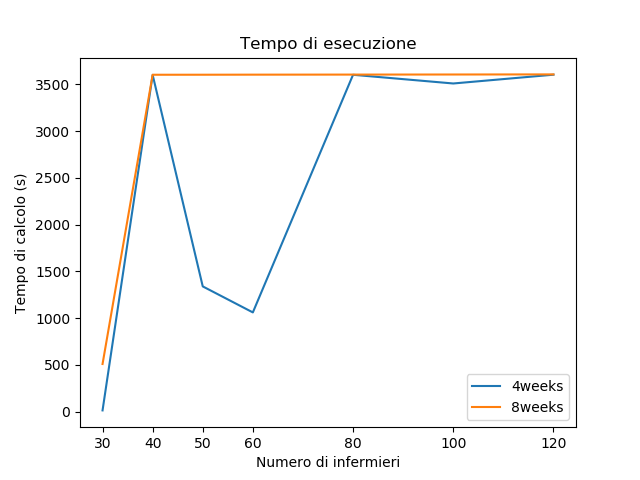
\includegraphics[scale=0.5]{img/Problema1/Time_1h-h0_w0.png}\\
  \caption{Tempo di esecuzione Problema 1}
\end{center}
\end{figure}

\begin{figure}[H]
\begin{center}
  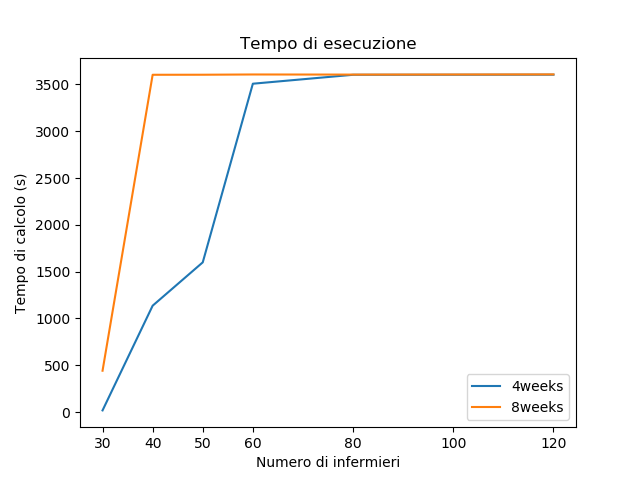
\includegraphics[scale=0.5]{img/Problema2/Time_1h-h0_w4.png}\\
  \caption{Tempo di esecuzione Problema 2}
\end{center}
\end{figure}

\begin{figure}[H]
\begin{center}
  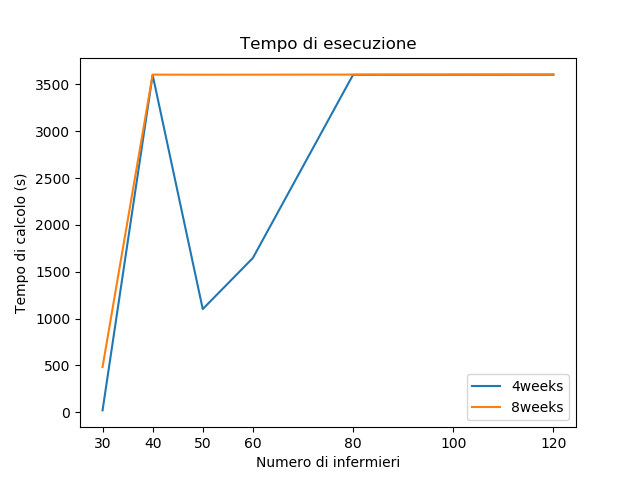
\includegraphics[scale=0.5]{img/Problema3/Time_1h-h1_w0.png}\\
  \caption{Tempo di esecuzione Problema 3}
\end{center}
\end{figure}

\begin{figure}[H]
\begin{center}
  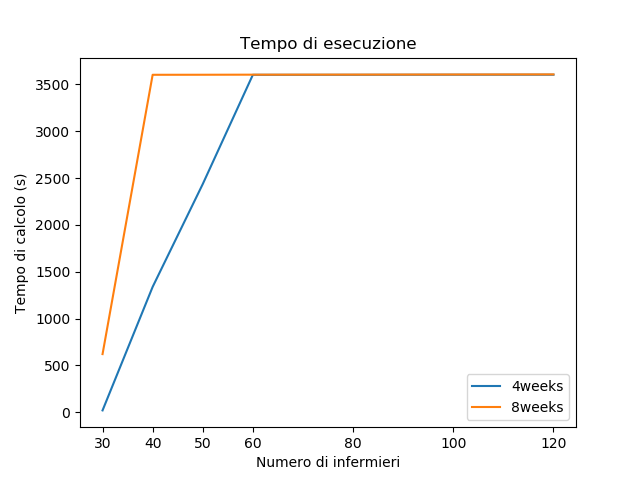
\includegraphics[scale=0.5]{img/Problema4/Time_1h-h1_w4.png}\\
  \caption{Tempo di esecuzione Problema 4}
\end{center}
\end{figure}


\subsection{Gap percentuale}
Di seguito si riportano i grafici nei quali si mostra il Gap percentuale del problema, dove si è posto un limite al tempo massimo di calcolo pari a 2 ore.
\begin{figure}[H]
\begin{center}
  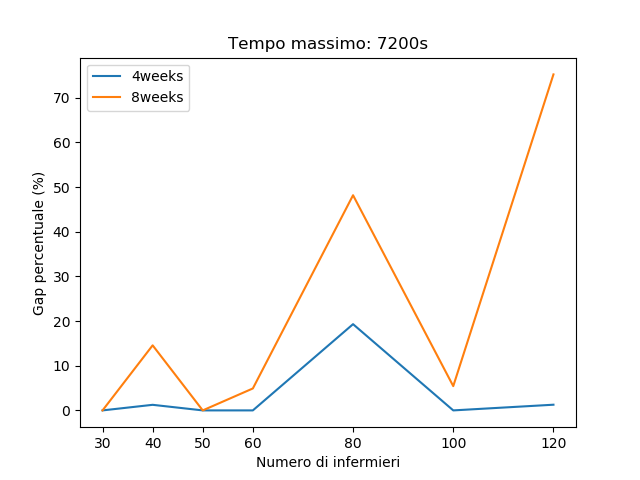
\includegraphics[scale=0.5]{img/Problema1/Gap_2h-h0_w0.png}\\
  \caption{Gap Problema 1}
\end{center}
\end{figure}

\begin{figure}[H]
\begin{center}
  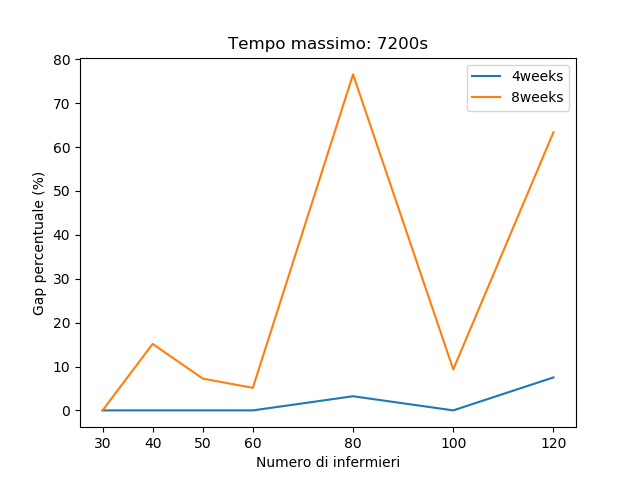
\includegraphics[scale=0.5]{img/Problema2/Gap_2h-h0_w4.png}\\
  \caption{Gap Problema 2}
\end{center}
\end{figure}

\begin{figure}[H]
\begin{center}
  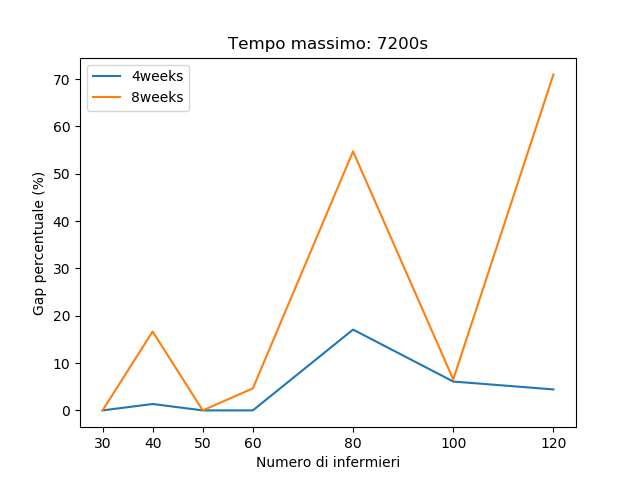
\includegraphics[scale=0.5]{img/Problema3/Gap_2h-h1_w0.png}\\
  \caption{Gap Problema 3}
\end{center}
\end{figure}

\begin{figure}[H]
\begin{center}
  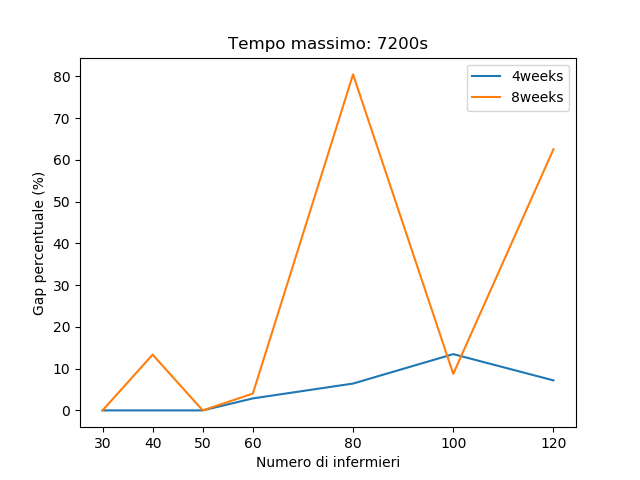
\includegraphics[scale=0.5]{img/Problema4/Gap_2h-h1_w4.png}\\
  \caption{Gap Problema 4}
\end{center}
\end{figure}

\newpage 
\section{Risultati}
Analizzando i grafici si possono fare le seguenti osservazioni:
\begin{itemize}
\item Il problema da 8 settimane appare molto più complesso da risolvere rispetto a quello di 4 settimane;
\item Il Gap del problema da 4 settimane non supera mai il 20\%;
\item Il Gap del problema da 8 settimane non supera mai l'80\%;
\item Il tempo di calcolo della soluzione arriva spesso in saturazione.
\end{itemize}

È necessario precisare che per eseguire una sperimentazione più precisa sarebbe stato opportuno fare una quantità maggiore di esperimenti facendo una media tra essi.

Si noti che, comunque, in tutti gli esperimenti fatti entro il tempo massimo, si riesce sempre a trovare una \textbf{soluzione} \textbf{ammissibile}.